\documentclass[tikz,border=2pt]{standalone}
\usepackage{amsmath}
\usetikzlibrary{arrows.meta,decorations.pathreplacing}
\begin{document}
% Anatomy of own_sum <- function(xvec) { ... return(out) }: name, reserved word, argument,
% body and return value; the call own_sum(1:10) returns 55.
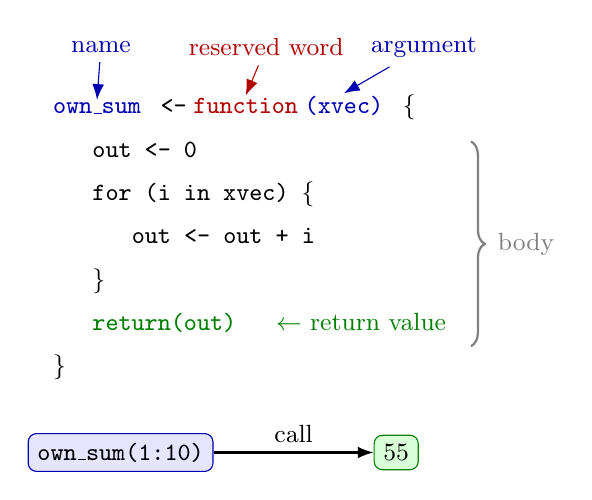
\begin{tikzpicture}[font=\small, >={Latex[length=2mm]},
  code/.style={anchor=base west, inner sep=1pt, font=\small\ttfamily}]
  % line 1, split into parts
  \node[code, text=blue!70!black] (nm) at (0,0) {own\_sum};
  \node[code] (as) at (nm.base east) {\ <-\ };
  \node[code, text=red!70!black] (fn) at (as.base east) {function};
  \node[code, text=blue!70!black] (ar) at (fn.base east) {(xvec)};
  \node[code] at (ar.base east) {\ \{};
  % body lines
  \node[code] (b1) at (0.5,-0.55) {out <- 0};
  \node[code] (b2) at (0.5,-1.10) {for (i in xvec) \{};
  \node[code] (b3) at (1.0,-1.65) {out <- out + i};
  \node[code] (b4) at (0.5,-2.20) {\}};
  \node[code, text=green!50!black] (b5) at (0.5,-2.75) {return(out)};
  \node[code] (b6) at (0,-3.30) {\}};
  % labels above line 1
  \node[blue!70!black] (lnm) at (0.65,0.85) {name};
  \node[red!70!black] (lfn) at (2.75,0.85) {reserved word};
  \node[blue!70!black] (lar) at (4.75,0.85) {argument};
  \draw[->, thin, blue!70!black] (lnm) -- (nm.north);
  \draw[->, thin, red!70!black] (lfn) -- (fn.north);
  \draw[->, thin, blue!70!black] (lar) -- (ar.north);
  % body brace
  \draw[decorate, decoration={brace, amplitude=5pt}, thick, gray] (5.35,-0.35) -- (5.35,-2.95)
     node[midway, right=6pt, gray] {body};
  % return value
  % call
  \node[draw=blue!70!black, fill=blue!10, rounded corners=3pt, font=\small\ttfamily] (call) at (0.9,-4.3) {own\_sum(1:10)};
  \node[draw=green!50!black, fill=green!15, rounded corners=3pt] (res) at (4.4,-4.3) {55};
  \draw[->, thick] (call) -- node[above] {call} (res);
  \node[green!50!black, anchor=base west] at (2.75,-2.75) {$\leftarrow$ return value};
\end{tikzpicture}
\end{document}
